%%%%%%%%%%%%%%%%%%%%%%%%%%%%%%%%%%%%%%%%%
% University/School Laboratory Report
% LaTeX Template
% Version 4.0 (March 21, 2022)
%
% This template originates from:
% https://www.LaTeXTemplates.com
%
% Authors:
% Vel (vel@latextemplates.com)
% Linux and Unix Users Group at Virginia Tech Wiki
%
% License:
% CC BY-NC-SA 4.0 (https://creativecommons.org/licenses/by-nc-sa/4.0/)
%
%%%%%%%%%%%%%%%%%%%%%%%%%%%%%%%%%%%%%%%%%

%----------------------------------------------------------------------------------------
%	PACKAGES AND DOCUMENT CONFIGURATIONS
%----------------------------------------------------------------------------------------

\documentclass[
	letterpaper, % Paper size, specify a4paper (A4) or letterpaper (US letter)
	10pt, % Default font size, specify 10pt, 11pt or 12pt
]{CSUniSchoolLabReport}

\addbibresource{sample.bib} % Bibliography file (located in the same folder as the template)

%----------------------------------------------------------------------------------------
%	REPORT INFORMATION
%----------------------------------------------------------------------------------------

\title{Computer Graphics Coursework 1 Report} % Report title

\author{Brooklyn Mcswiney} % Author name(s), add additional authors like: '\& James \textsc{Smith}'

\date{ }
%----------------------------------------------------------------------------------------

\begin{document}

\maketitle % Insert the title, author and date using the information specified above

\noindent\makebox[\linewidth]{\rule{\paperwidth}{0.4pt}}

\tableofcontents

\pagebreak
%----------------------------------------------------------------------------------------
%	OBJECTIVE
%----------------------------------------------------------------------------------------

\section{Implementation}

\subsection{Drawing Pixels}

Within the window the coordinates count from the top left of the window
to the bottom right. This means that the pixel (0, 0) is in the top left
corner, (w-1, 0) is in the top right corner and (0, h-1) is in the 
bottom left corner.

\begin{figure}[h]
	\centering
	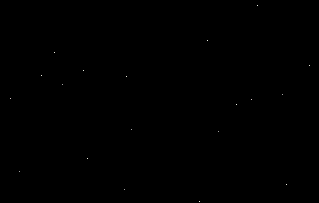
\includegraphics[scale=0.6]{particleFieldZoom}
	\caption{Particle field from the project implementation}
\end{figure}

\subsection{Drawing Lines}
\begin{flushleft}
	The line implementation works by starting with two points. The start and
	end of the line. The program will then take these values and calculate 2
	numbers \(d_x\) and \( d_y\). Then, the program will find which axis the
	line moves the most along (Known as the X or Y major). This is done through
	seeing which value between \(d_x\) and \( d_y\) is the greatest. Should \(d_x\)
	be greater we step along the X axis. The same is true should \(d_y\) be greater.
	The program then keeps track of this by saving a `step' variable as the corresponding 
	major.
\end{flushleft}

\begin{flushleft}
	The final step before moving onto deciding which pixels get drawn is to calculate
	the increase required each iteration in the \(x\) and \(y\) directions.
	This increase is found by dividing \(d_x\) and \(dy\) by the step variable that was
	saved earlier. 
\end{flushleft}

\begin{flushleft}
	In order to draw the line the program now iterates over as many `steps'
	needed to draw the line from the start to the end. During each iteration
	the program will check that the pixel is within the bounds of the surface
	and should this check return true the pixel will be drawn. This is done to 
	avoid out of bounds errors within the program. The last stage of the loop is 
	to move to the next pixel in the line by adding the \(x\) and \(y\) increase 
	to our current pixel location. (\cite{Kamble:2021})
\end{flushleft}



\begin{figure}[H]
	\centering
	\begin{minipage}[b]{0.4\textwidth}
		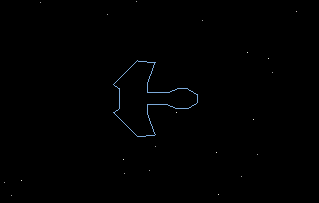
\includegraphics[width=\textwidth]{ship}
		\caption{Ship drawn.}
	\end{minipage}
	\hfill
	\begin{minipage}[b]{0.4\textwidth}
		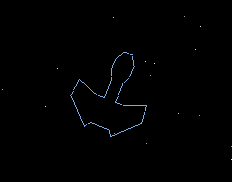
\includegraphics[width=\textwidth]{shipRotate}
		\caption{Ship rotated}
  	\end{minipage}
\end{figure}

\subsection{Drawing Triangles}
\begin{flushleft}
	This algorithm begins by finding the possible bounds of the triangle by 
	iterating through the points given to find the maximum and minimum coordinates. 
	Once the bounds of the triangle are discovered the program will iterate 
	through every pixel within the bounds. Every loop the program will check 
	if the current pixel (\(X\)) is within the triangle by performing 3 half-plane tests.
	These tests are performed using the following algorithm \(F(X)=n \cdot (X - P)\).
	Should \(F(X) > 0\) be true for any of the lines the program continues onto 
	the next pixel. Should the pixel pass all the half-plane tests the program will 
	then check the pixel is within the window and if it is the pixel gets drawn. 

\end{flushleft}

\subsection{Barycentric Interpolation}
\begin{flushleft}
	The algorithm begins exactly the same as the previous triangle algorithm, by 
	finding the bounds of the triangle to be drawn. The algorithm then loops through
	this rectangle and performs calculations to determine whether or not a pixel is within
	the triangle to be drawn. The changes from the previous algorithm begin with these checks.
	These checks involve finding \(\alpha\), \(\beta\) and \(\gamma\) values for a given point.
	These values are known as Barycentric Coordinates and can be found for any given point (\(U\))
	on a triangle.
\end{flushleft}
\begin{flushleft}
	Given a triangle with points \(A\), \(B\) and \(C\) the program need to find the vectors \(u = B-A\) and \(y = C-A\).
	Once these two vectors have been found the program then uses the following formula to find the area of the triangle \(ABC\).
\end{flushleft}
\begin{align*}
	area(ABC) = \frac{(u_{x} \times v_{y}) - (u_{y} \times v_{x})}{2}
\end{align*}
\begin{flushleft}
	The code can then call a function for this formula for each of the three sub triangles. Once each sub area has 
	been calculated the program can then perform the following formulas to find the values of \(\alpha\), \(\beta\) and \(\gamma\).
\end{flushleft}
\begin{align*}
	\alpha = \frac{area(BCU)}{area(ABC)}, \beta = \frac{area(AUC)}{area(ABC)}, \gamma = \frac{area(ABU)}{area(ABC)}
\end{align*}
\pagebreak
\begin{flushleft}
	Finally, should each of these values be between 0 and 1 the algorithm will draw a pixel at the given point.
	This pixel shall be a colour interpolated from the three points on the triangle using the following formula 
	for each RGB value.
\end{flushleft}
\begin{align*}
	colour = A_{colour} \times \alpha + B_{colour} \times \beta + C_{colour} \times \gamma
\end{align*}
\begin{figure}[H]
	\centering
	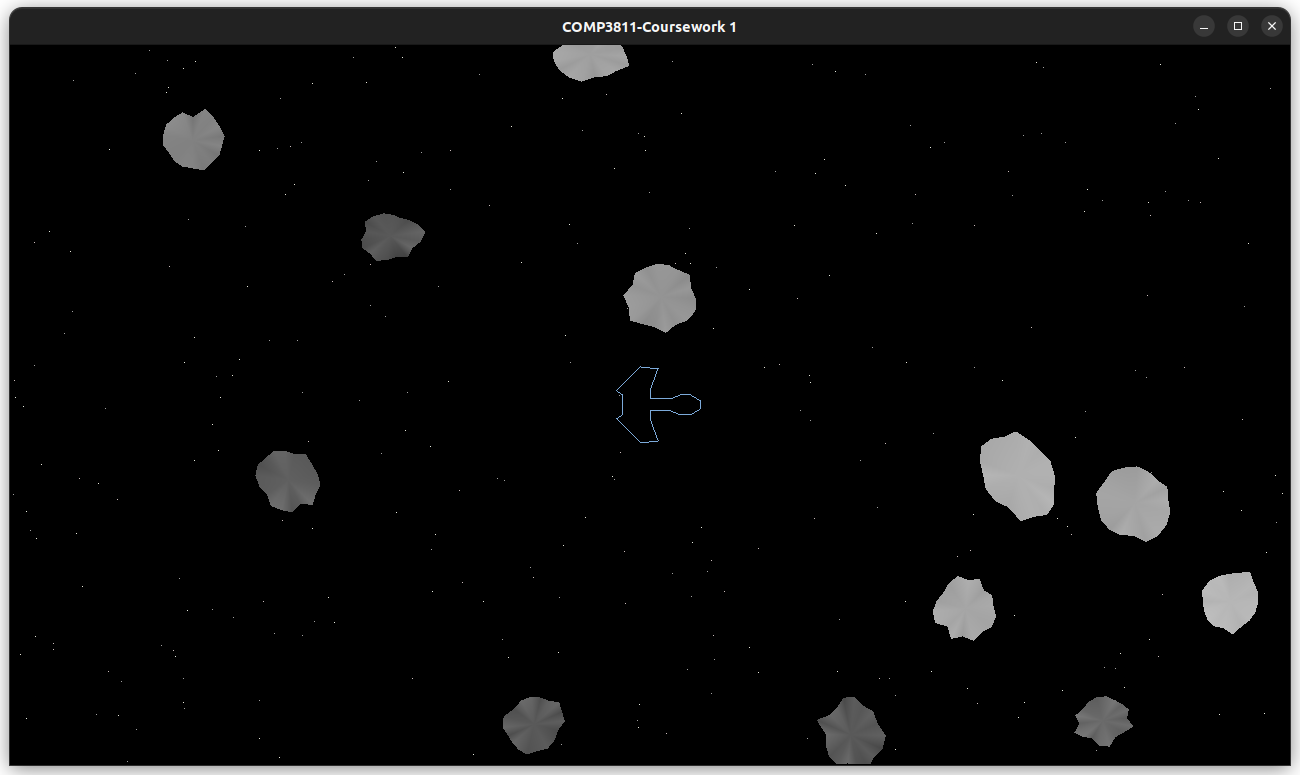
\includegraphics[width=0.6\textwidth]{interpol.png}
	\caption{Asteroids drawn using Barycentric Interpolation}
\end{figure}

\subsection{Blitting Images}
\subsection*{Helper Algorithims}
\begin{flushleft}
	These helper algorithms differ slightly from the ones used in order to set pixels. This is due to the fact that
	they use RGBA representation as opposed to RGBx representations. This means that as well as returning the RGB values
	when getting a pixel the program must also return an A value. This A value is used to indicate the opacity of a pixel 
	which is then later used to check whether a pixel should or should not be drawn on the surface from the image.
\end{flushleft}
\subsection*{Main Blitting Algorithm}
\begin{flushleft}
	The blitting algorithm begins by starting a loop through the image to be rendered. Within this loop 
	the program first finds the current position on the surface by adding the starting position to the x and y
	values being used to loop through the image. The algorithm then calls the helper algorithm to get a pixel from the image.
	The program then checks if the current pixel should be masked or not by checking if the A value is greater than 0. The program
	then makes sure that the current pixel is within the bounds of the surface and if it is the pixel gets drawn onto the surface.
\end{flushleft}
\begin{flushleft}
	One possible optimisation that could be made is improving the clipping of the image. For example, currently the program will check every 
	pixel outside the bounds of the surface even if no more pixels could possibly be on the surface. This could be further optimised
	by stopping the current loop if the following pixels will always be outside the borders of the surface.
\end{flushleft}
\section{Testing}
\subsection{Testing: Lines}
\subsection*{Test 1 {-} Drawing multiple directions off screen}
This test was implemented as it is important that the program can handle lines 
being drawn off screen no matter the direction. Currently the tests only check for 
1 direction off screen so I decided to expand on that to all directions. Furthermore, 
if the program cannot handle lines being drawn off screen the program will most likely
crash which is unacceptable.

\subsection*{Test 2 {-} Two connected lines}
This test was implemented in order to ensure there's no pixel gaps when two lines 
are drawn next to each other. This is a desireable effect as when drawing more 
complex shapes using lines we must ensure the program will not leave any gaps while
drawing.


\subsection*{Test 3 {-} Two lines running parallel next to each other}
This test was implemented to ensure no gaps are present when lines are parallel to each other.
This is desireable for the same reason as the previous test. That reason being, 
when drawing more complex shapes with lines we want to ensure no gaps are present.
\subsection*{Test 4 {-} Two lines overlapping}
This test was implemented to ensure that a second line drawn after another line in The
same place would overwrite the previous line. This feature is important as some animations
 will require changes in pixels so it is important pixels drawn later can fully overwrite
 previous pixels.
\subsection*{Test 5 {-} Whole screen drawn onto}
This test ensures that every pixel within a surface can be drawn onto. This is important
as we want to make sure that every pixel can be used. This also ensures that any bug 
related to drawing to specific pixels can be identified and fixed.

\subsection*{Visualisations}
\begin{figure}[H]
	\centering
	\begin{minipage}[b]{0.4\textwidth}
		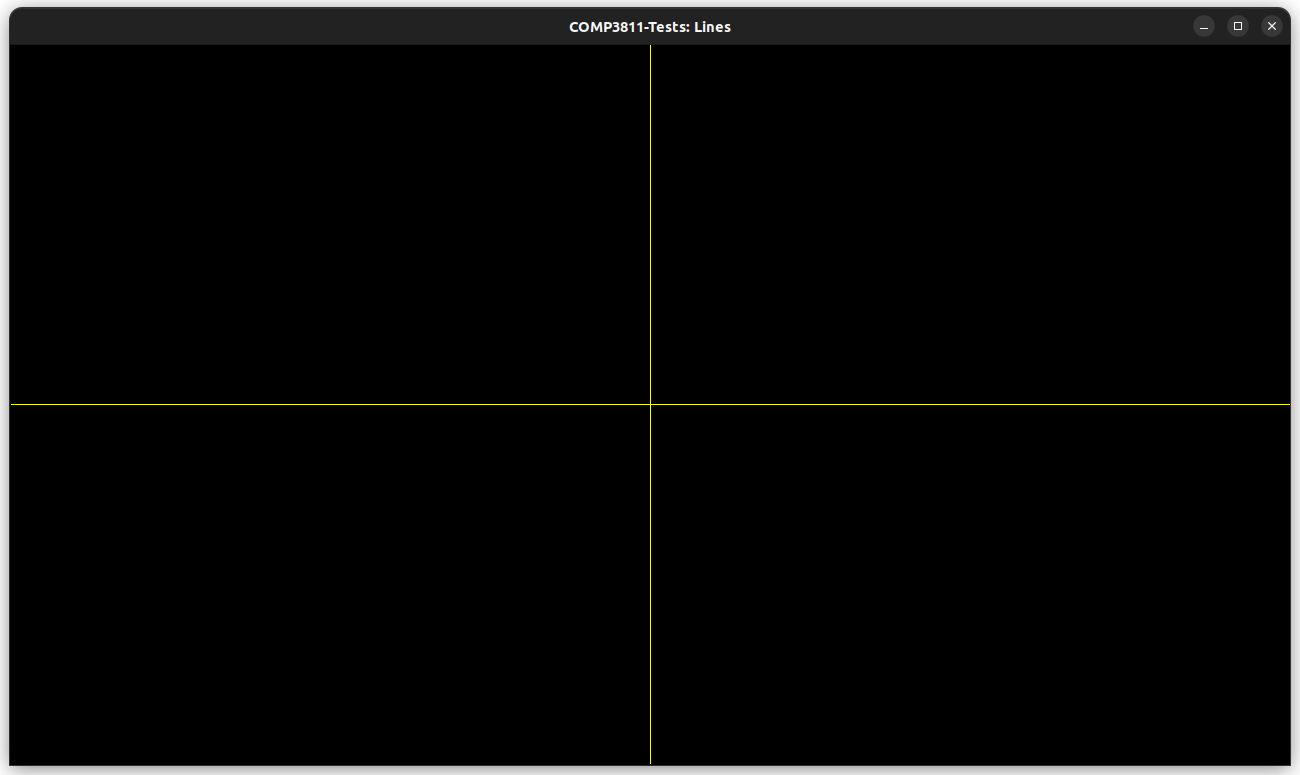
\includegraphics[width=\textwidth]{offscreen2}
		\caption{Demostration of test 1 using lines sandbox.}
	\end{minipage}
	\hfill
	\begin{minipage}[b]{0.4\textwidth}
		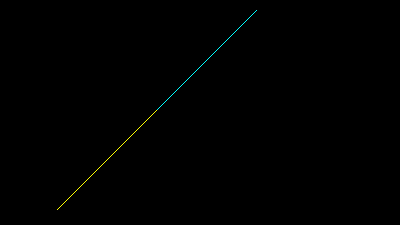
\includegraphics[width=\textwidth]{2connected}
		\caption{Demostration of test 2 using lines sandbox}
  	\end{minipage}
\end{figure}
\begin{figure}[H]
	\centering
	\begin{minipage}[b]{0.4\textwidth}
		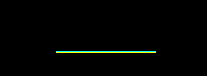
\includegraphics[width=\textwidth]{2ontop}
		\caption{Demostration of test 3 using lines sandbox}
	\end{minipage}
	\hfill
	\begin{minipage}[b]{0.4\textwidth}
		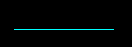
\includegraphics[width=\textwidth]{2over}
		\caption{Demostration of test 4 using lines sandbox}
  	\end{minipage}
\end{figure}
\begin{figure}[H]
	\centering
	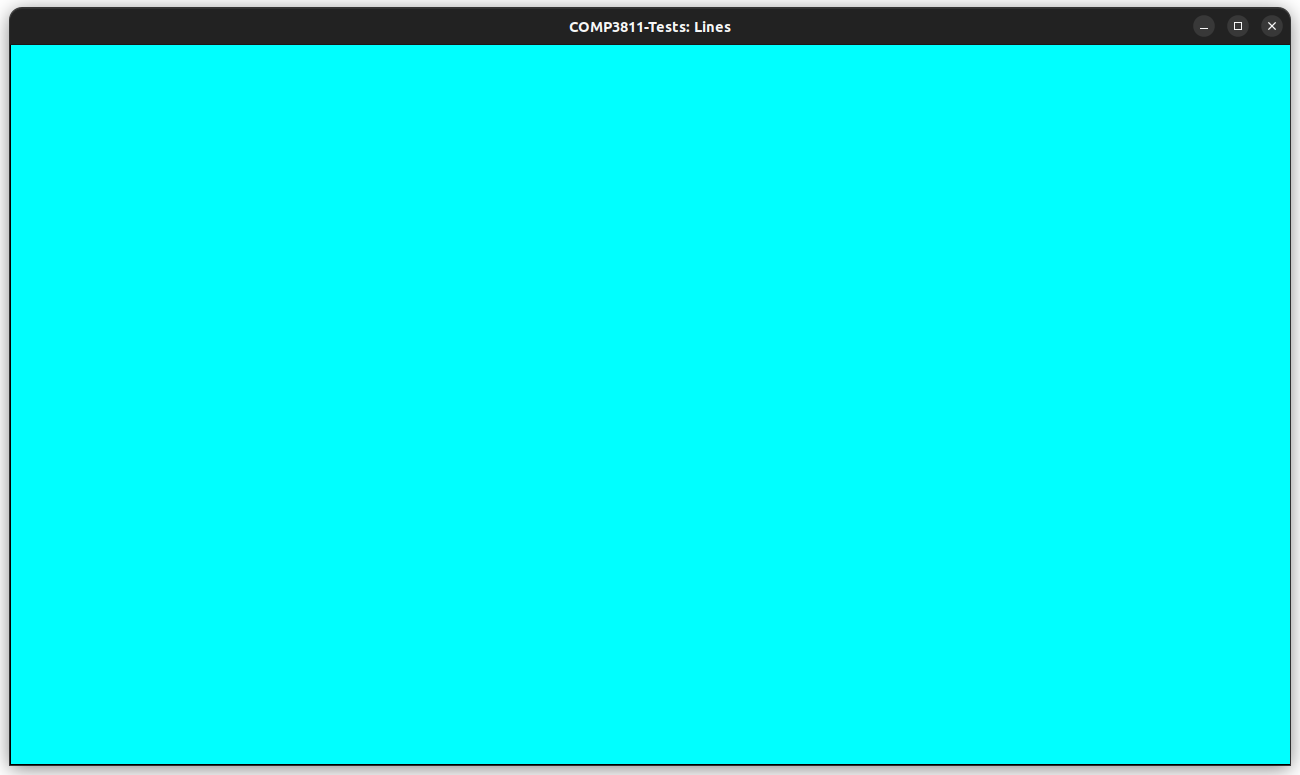
\includegraphics[width=0.3\textwidth]{fullscreen}
	\caption{Demostration of test 5 using lines sandbox}	
\end{figure}
\subsection{Testing: Triangles}
\subsection*{Test 1 {-} Flat triangle}
For this test we want to ensure that drawing a flat triangle just draws a line on the surface.
This could be useful for certain animations that involve a triangle morphing in order to be flatter. 
This test ensures that the triangle does not disappear early during this animation.
\subsection*{Test 2 {-} Any point order}
This test ensures that no matter what order the points are inputted the triangle is still drawn.
This is useful as due to rotation there is no way to know what order the points of the triangle will 
arrive in. Therefore this test exists to ensures the drawing algorithm accounts for this.
\subsection*{Test 3 {-} Triangles drawn outside}
This test ensures the program does not crash when an entire triangle is drawn outside the bounds of 
the screen. This is useful as for certain things (such as objects in a video game for example) a user 
may want to keep track of things even if they are not within the bounds of the screen. This program 
should be able to handle this.

\section{Benchmarks}
\subsection{Computer Information}
\begin{flushleft}
	All tests were performed using an 11th generation intel core i3\-1115G4.
	The CPU has 4 caches present: a data cache with 48KiB, an instruction cache with 32KiB,
	and two unified cahces. One unified cache has 1280KiB, the other has 6144KiB.
	The computer the tests were performed on also has access to 8gb of RAM.
\end{flushleft}
\subsection{Blitting}
\begin{table}[ht]
	\caption{Blitting Benchmark Results} % title of Table
	\centering 
	\begin{tabular}{c c c c c} 
	\hline
	Method name & surface size & Time(ns) & CPU(ns) & Iteraions \\ [0.5ex] 
	\hline
	alpha masking & 320x240 & 3,831,941 & 3,815,423 & 176 \\ 
	alpha masking & 7680x4320 & 5,756,367 & 5,729,355 & 125 \\
	no alpha masking & 320x240 & 3,953,626 & 3,946,029 & 178 \\
	no alpha masking & 7680x4320 & 7,282,696 & 7,257,732 & 94 \\
	\verb|std::memcpy| & 320x240 & 226,571 & 224,768 & 3,272 \\ 
	\verb|std::memcpy| & 7680x4320 & 232,251 & 230,998 & 3,122 \\[1ex] 
	\end{tabular}
\end{table}
\begin{flushleft}
	From this data I can see that the fastest algorithm in terms of time taken is 
	clearly blitting through the use of \verb|std::memcpy|. This is most likely due
	to the algorithm involving \verb|std::memcpy| only containing one \verb|for| loop.
	This algorithm achieves this through directly copying every row of the image onto
	the surface from a specified point. Another benefit of this algorithm that can be seen from 
	the data is that it scales well with larger images. This effect is also due to the algorithm
	only having one \verb|for| loop as opposed to two.
\end{flushleft}
\begin{flushleft}
	This data also seems to indicate that blitting with alpha masking is faster than
	blitting with alpha masking. The most likely reason for this is due to my implementation 
	of clipping. Clipping is performed by checking is a pixel is in bounds right before it
	is about to be drawn. When alpha masking is performed this (relatively expensive) check 
	is skipped for every pixel that is to be masked. On the other hand, if alpha masking is not 
	performed this check is done for every pixel in the bounds of the image. Should this clipping 
	check be moved to a place in which it's performed no matter whether alpha masking is present or not
	I expect blitting with no alpha mask to be slightly faster as there is one less check to perform.
\end{flushleft}
\subsection{Line drawing}
\begin{table}[!htb]
    \caption{Line Benchmark Results}
    \begin{minipage}{.5\linewidth}
      \caption{DDA Results}
      \centering
        \begin{tabular}{c c c c}
            Test & surface size & Time(ns) & Iteraions \\ [0.5ex]
			\hline
			Diagonal & 320x240 & 1,667 & 358,427 \\
			Diagonal & 7680x4320 & 53,748 & 12,640 \\
			Horizontal & 320x240 & 1,020 & 628,431  \\
			Horizontal & 7680x4320 & 24,398 & 29,017 \\
			Fullscreen & 320x240 & 451,847 & 1,277 \\
			Fullscreen & 7680x4320 & 170,828,342 & 4 \\
        \end{tabular}
    \end{minipage}%
	\vline
    \begin{minipage}{.5\linewidth}
      \centering
        \caption{Bresenham Results}
        \begin{tabular}{c c c c}
            Test & surface size & Time(ns) & Iteraions \\ [0.5ex]
			\hline
			Diagonal & 320x240 & 3,173 & 213,402 \\
			Diagonal & 7680x4320 & 77,639 & 8,978 \\
			Horizontal & 320x240 & 1,905 & 354,100 \\
			Horizontal & 7680x4320 & 45,958 & 15,184 \\
			Fullscreen & 320x240 & 772,071 & 817 \\
			Fullscreen & 7680x4320 & 335,260,630 & 2 \\
        \end{tabular}
    \end{minipage} 
\end{table}
(\cite{Madan:2014})
\section{My own spaceship}

\subsection*{}
%----------------------------------------------------------------------------------------
%	BIBLIOGRAPHY
%----------------------------------------------------------------------------------------

\printbibliography% Output the bibliography

%----------------------------------------------------------------------------------------

\end{document}